\chapter{Evaluation}

In order to evaluate the effectiveness of CRAFTS' prediction methods, we run each of them on the workloads outlined in \Cref{ch:workloads}. At the beginning of each experiment, the tuner is run on the baseline workload to tune the parameters of the prediction algorithm. This is done to ensure that the tuning is done with minimal anomalies present. This will allow us to see how the prediction methods handle anomalous traffic under regular conditions. The effectiveness of each algorithm is measured using root mean squared deviation (RMSD), as discussed in \Cref{eq:rmsd}. We further break the results down into over-estimations and under-estimations, giving the RMSD for each as well as the percent of predictions which fell into each category. Each of the following sections will discuss how each predictor was evaluated and analyze their performance.

\section{Translation}
The translation predictor uses each week as the training set for the following week's predictions. The results of each week are then combined to create a single error measurement.

We can see in \Cref{fig:translation_outage} how the translation predictor baseline is not tolerant to outages. The outage is directly replayed onto the next week which negatively influences our predictions. Similarly, we can see how anomalous spikes cause a similar effect in \Cref{fig:translation_spike}.

\begin{figure}
\centering
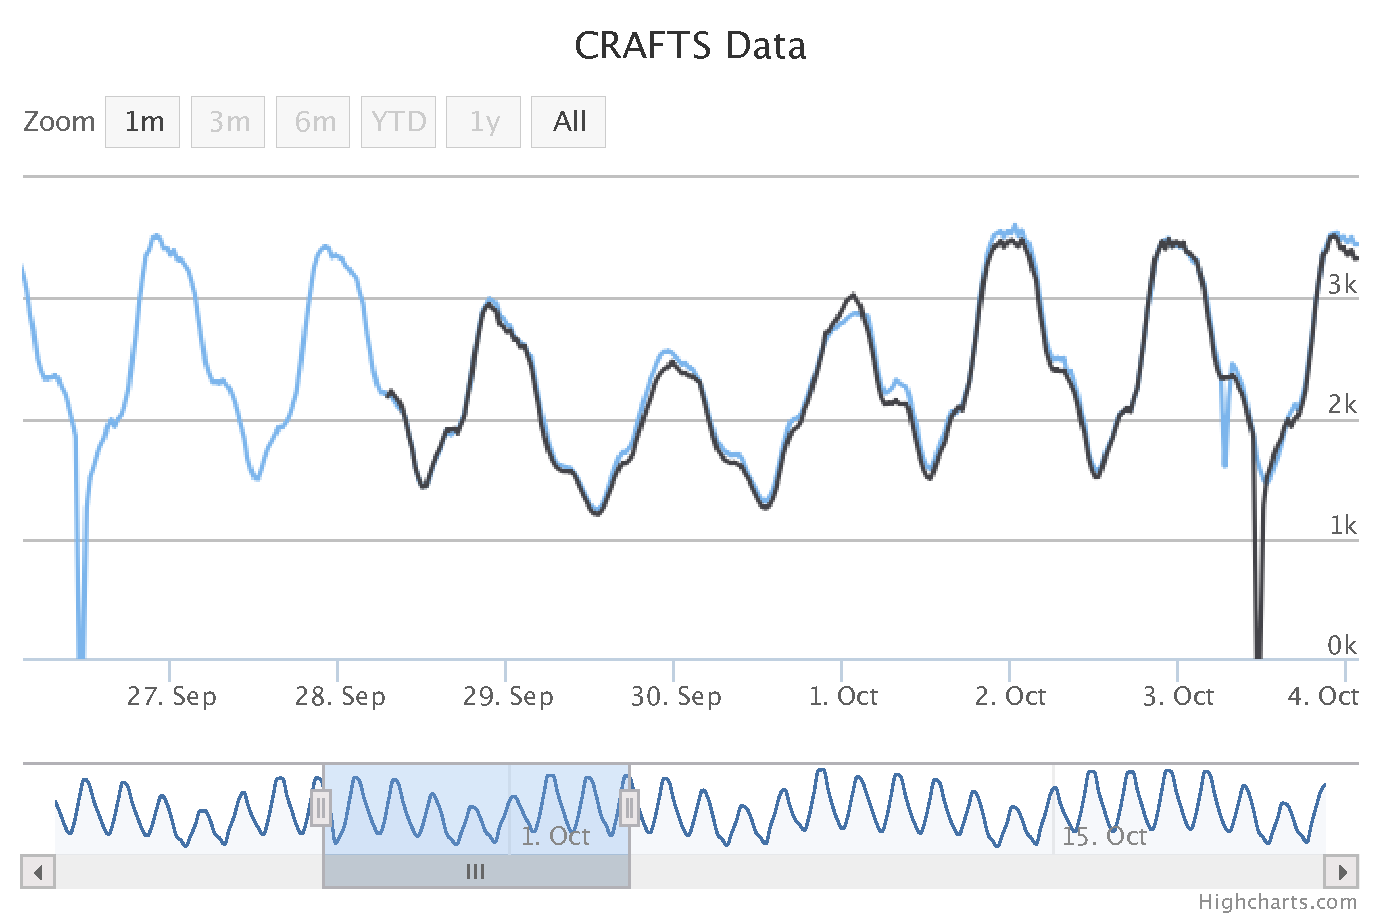
\includegraphics[width=\textwidth]{results/graphs/translation_outage.pdf}
\caption{An outage translated by the translation predictor}
\label{fig:translation_outage}
\end{figure}

\begin{figure}
\centering
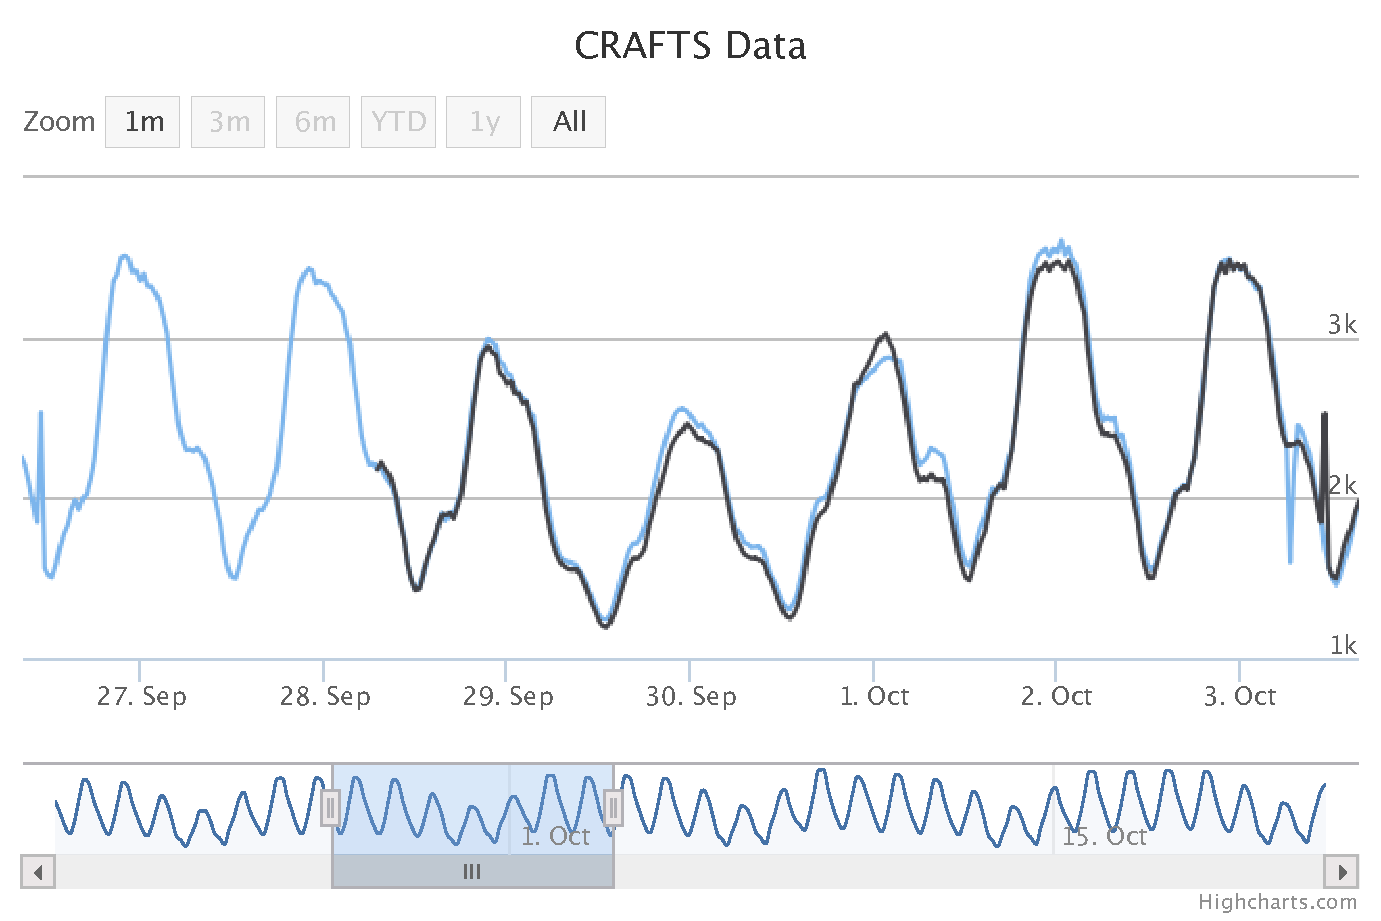
\includegraphics[width=\textwidth]{results/graphs/translation_spike.pdf}
\caption{A usage spike translated by the translation predictor}
\label{fig:translation_spike}
\end{figure}

\begin{table}[H]
\centering
\begin{tabular}{| l | l | l |}
\hline
Type & RMSD & Percent \\ \hline
Under & 113 & 68.7\% \\ \hline
Over & 76 & 31.3\% \\ \hline
Total & 103 & \\ \hline
\end{tabular}
\caption{Translation predictor results for the baseline workload}
\end{table}

% Outage workloads

\begin{table}[H]
\centering
\begin{tabular}{| l | l | l |}
\hline
Type & RMSD & Percent \\ \hline
Under & 122 & 68.7\% \\ \hline
Over & 76 & 31.3\% \\ \hline
Total & 110 & \\ \hline
\end{tabular}
\caption{Translation predictor results for the 10-minute outage workload}
\end{table}

\begin{table}[H]
\centering
\begin{tabular}{| l | l | l |}
\hline
Type & RMSD & Percent \\ \hline
Under & 132 & 68.8\% \\ \hline
Over & 76 & 31.2\% \\ \hline
Total & 117 & \\ \hline
\end{tabular}
\caption{Translation predictor results for the 30-minute outage workload}
\end{table}

\begin{table}[H]
\centering
\begin{tabular}{| l | l | l |}
\hline
Type & RMSD & Percent \\ \hline
Under & 145 & 68.9\% \\ \hline
Over & 76 & 31.1\% \\ \hline
Total & 127 & \\ \hline
\end{tabular}
\caption{Translation predictor results for the 60-minute outage workload}
\end{table}

% Spike workloads

\begin{table}[H]
\centering
\begin{tabular}{| l | l | l |}
\hline
Type & RMSD & Percent \\ \hline
Under & 113 & 68.7\% \\ \hline
Over & 83 & 31.3\% \\ \hline
Total & 105 & \\ \hline
\end{tabular}
\caption{predictor results for the low spike workload}
\end{table}

\begin{table}[H]
\centering
\begin{tabular}{| l | l | l |}
\hline
Type & RMSD & Percent \\ \hline
Under & 113 & 68.7\% \\ \hline
Over & 91 & 31.3\% \\ \hline
Total & 107 & \\ \hline
\end{tabular}
\caption{predictor results for the mid spike workload}
\end{table}

\begin{table}[H]
\centering
\begin{tabular}{| l | l | l |}
\hline
Type & RMSD & Percent \\ \hline
Under & 113 & 68.7\% \\ \hline
Over & 102 & 31.3\% \\ \hline
Total & 110 & \\ \hline
\end{tabular}
\caption{predictor results for the high spike workload}
\end{table}

\section{Fast Fourier Transform}
The fast Fourier transform predictor was evaluated in the same way as the translation predictor. In the baseline workload, the tuner found that filtering out 96\% of the weakest frequencies optimal.

While the spike workloads were easily handled by the FFT predictor, we saw issues in the outage workloads. Although we attempt to smooth the data, we still find that the outage can noticeable disruptions in this predictors results. Further tests show that if the outage had been included in the tuning, the tuner determined that 98\% was the optimal percentage of the weakest frequencies to filter out. When running the predictor with this value, the outage hardly affects the prediction. For this parameter, the tuner likely does more harm than good. We want to filter out as much noise as possible while still making accurate predictions. In this case, it would be more desirable to take a parameter which causes higher inaccuracy some of the time, but is resistant to outages. This represents a scenario which the current implementation of the tuner is unable to optimize.

\begin{table}[H]
\centering
\begin{tabular}{| l | l | l |}
\hline
Type & RMSD & Percent \\ \hline
Under & 140 & 76.2\% \\ \hline
Over & 61 & 23.8\% \\ \hline
Total & 125 & \\ \hline
\end{tabular}
\caption{FFT predictor results for the baseline workload}
\end{table}

\begin{figure}[H]
\centering
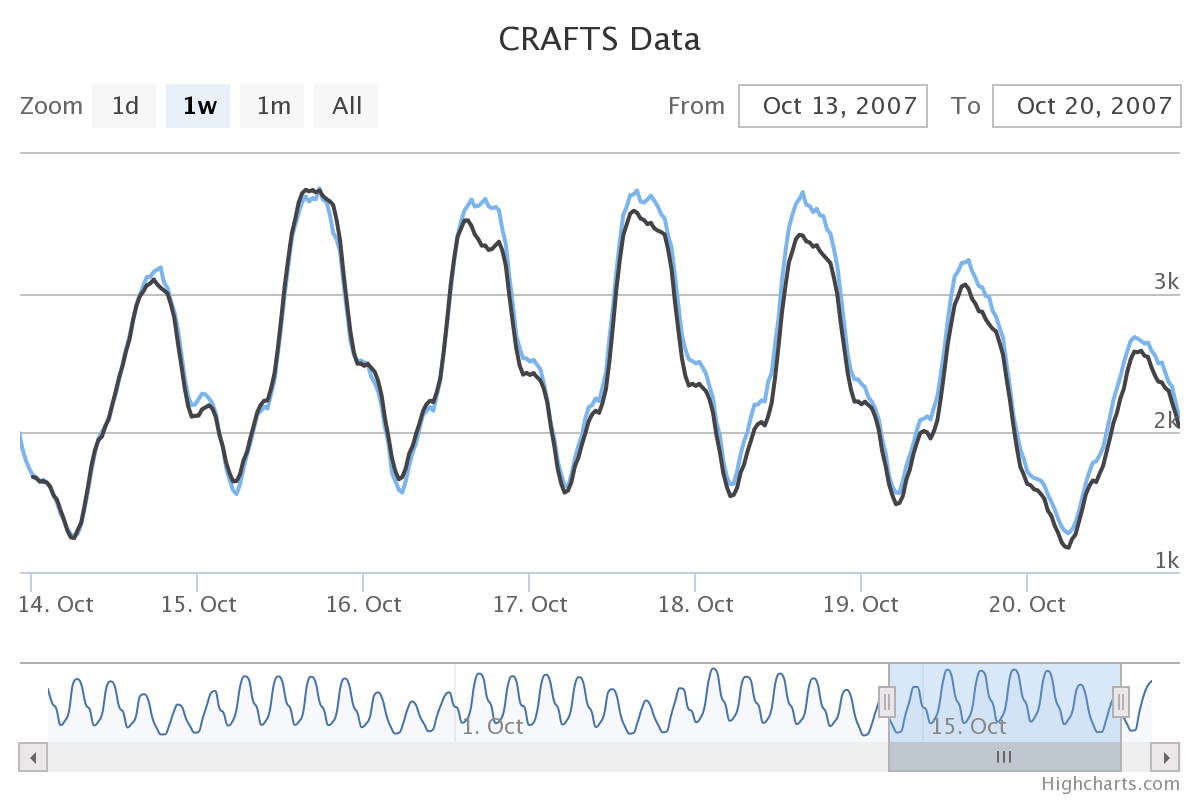
\includegraphics[width=\textwidth]{results/graphs/fft_baseline.png}
\caption{FFT prediction results for the baseline workload}
\label{fig:fft_b}
\end{figure}

\begin{table}[H]
\centering
\begin{tabular}{| l | l | l | l | l |}
\hline
Type & \multicolumn{2}{c |}{Regular} & \multicolumn{2}{c |}{Anomalous} \\ \hline
 & RMSD & Percent & RMSD & Percent \\ \hline
Under & 211 & 74.1\% & 1741 & 100.0\% \\ \hline
Over & 85 & 25.9\% & 0 & 0.0\% \\ \hline
Total & 186 & & 1741 & \\ \hline
\end{tabular}
\caption{FFT predictor results for the training outage workload with 96\% filtering}
\end{table}

\begin{figure}[H]
\centering
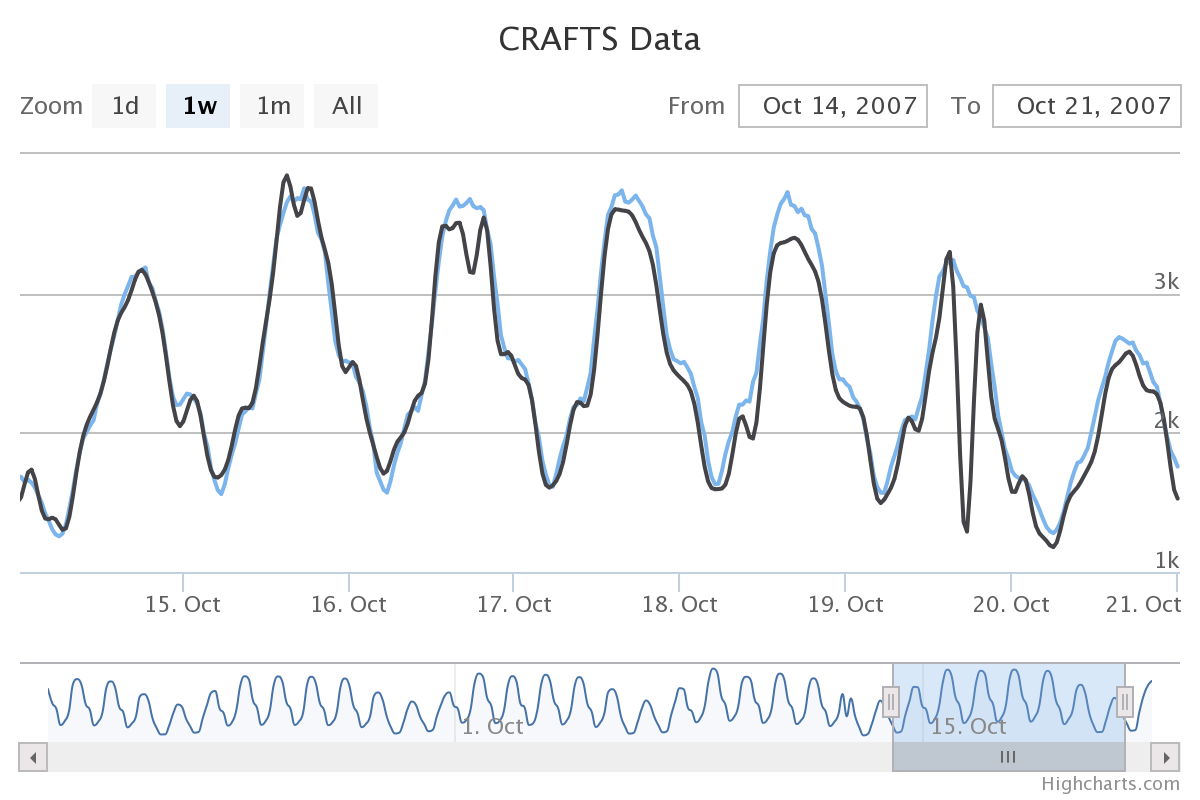
\includegraphics[width=\textwidth]{results/graphs/fft_training_outage_96.png}
\caption{FFT prediction results for the training outage workload with 96\% filtering}
\label{fig:fft_to96}
\end{figure}

\begin{table}[H]
\centering
\begin{tabular}{| l | l | l | l | l |}
\hline
Type & \multicolumn{2}{c |}{Regular} & \multicolumn{2}{c |}{Anomalous} \\ \hline
 & RMSD & Percent & RMSD & Percent \\ \hline
Under & 195 & 75.0\% & 721 & 100.0\% \\ \hline
Over & 88 & 25.0\% & 0 & 0.0\% \\ \hline
Total & 175 & & 721 & \\ \hline
\end{tabular}
\caption{FFT predictor results for the training outage workload with 99\% filtering}
\end{table}

\begin{figure}[H]
\centering
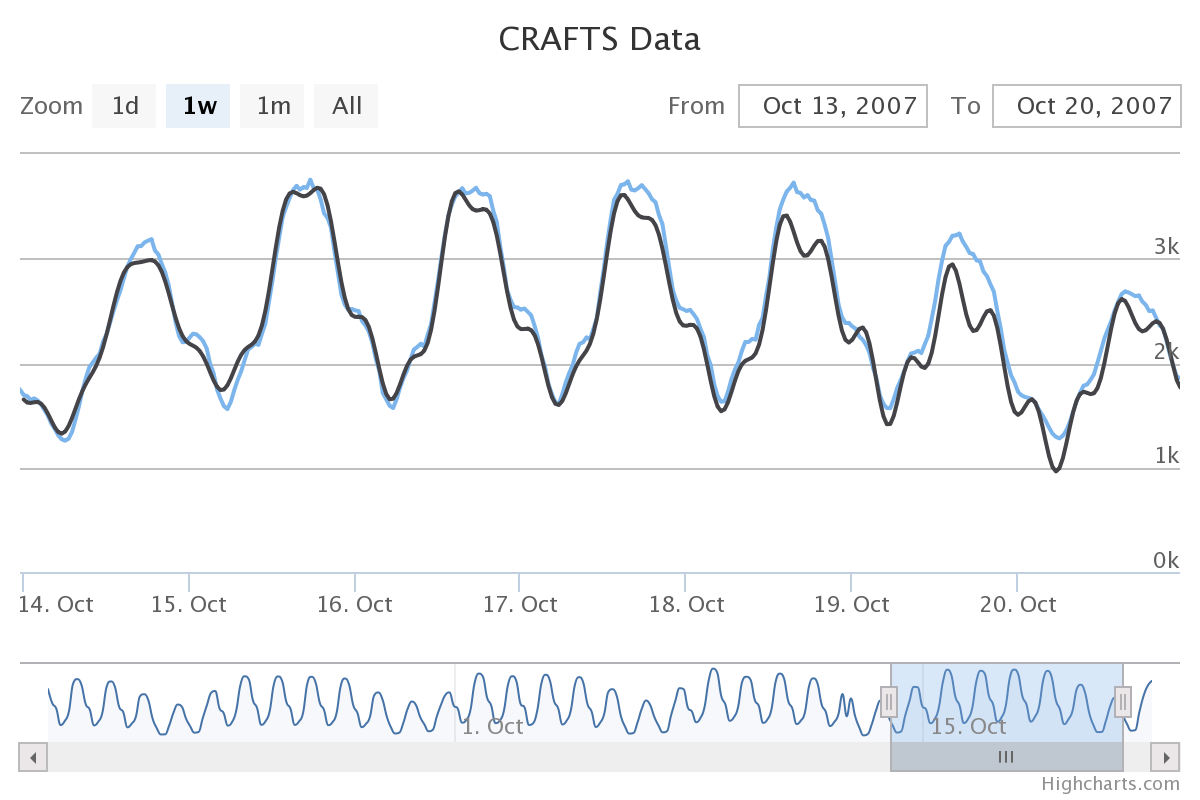
\includegraphics[width=\textwidth]{results/graphs/fft_training_outage_99.png}
\caption{FFT prediction results for the training outage workload with 99\% filtering}
\label{fig:fft_to99}
\end{figure}

\begin{table}[H]
\centering
\begin{tabular}{| l | l | l | l | l |}
\hline
Type & \multicolumn{2}{c |}{Regular} & \multicolumn{2}{c |}{Anomalous} \\ \hline
 & RMSD & Percent & RMSD & Percent \\ \hline
Under & 139 & 75.9\% & 0 & 0.0\% \\ \hline
Over & 194 & 24.1\% & 2869 & 100.0\% \\ \hline
Total & 154 & & 2869 & \\ \hline
\end{tabular}
\caption{FFT predictor results for the horizon outage workload}
\end{table}

\begin{figure}[H]
\centering
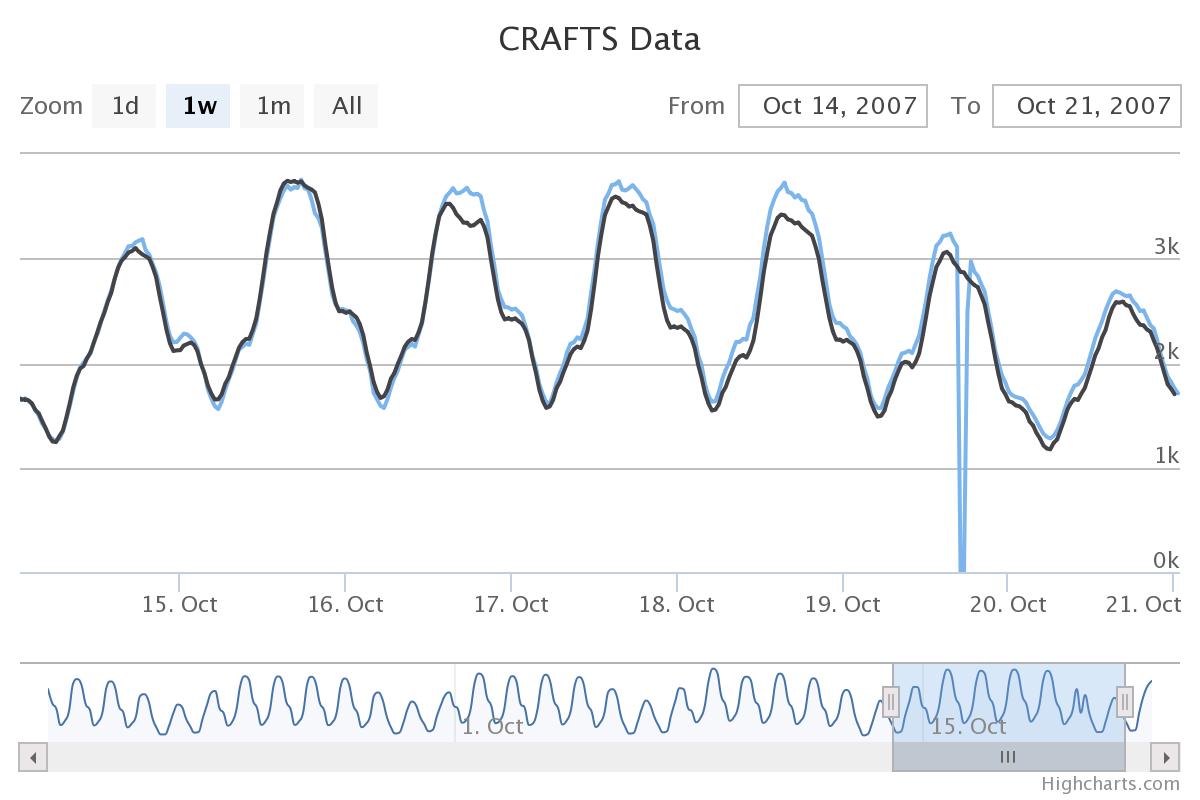
\includegraphics[width=\textwidth]{results/graphs/fft_horizon_outage.png}
\caption{FFT prediction results for the horizon outage workload}
\label{fig:fft_ho}
\end{figure}

\begin{table}[H]
\centering
\begin{tabular}{| l | l | l | l | l |}
\hline
Type & \multicolumn{2}{c |}{Regular} & \multicolumn{2}{c |}{Anomalous} \\ \hline
 & RMSD & Percent & RMSD & Percent \\ \hline
Under & 143 & 74.6\% & 0 & 0.0\% \\ \hline
Over & 86 & 25.4\% & 427 & 100.0\% \\ \hline
Total & 131 & & 427 & \\ \hline
\end{tabular}
\caption{FFT predictor results for the training spike workload}
\end{table}

\begin{figure}[H]
\centering
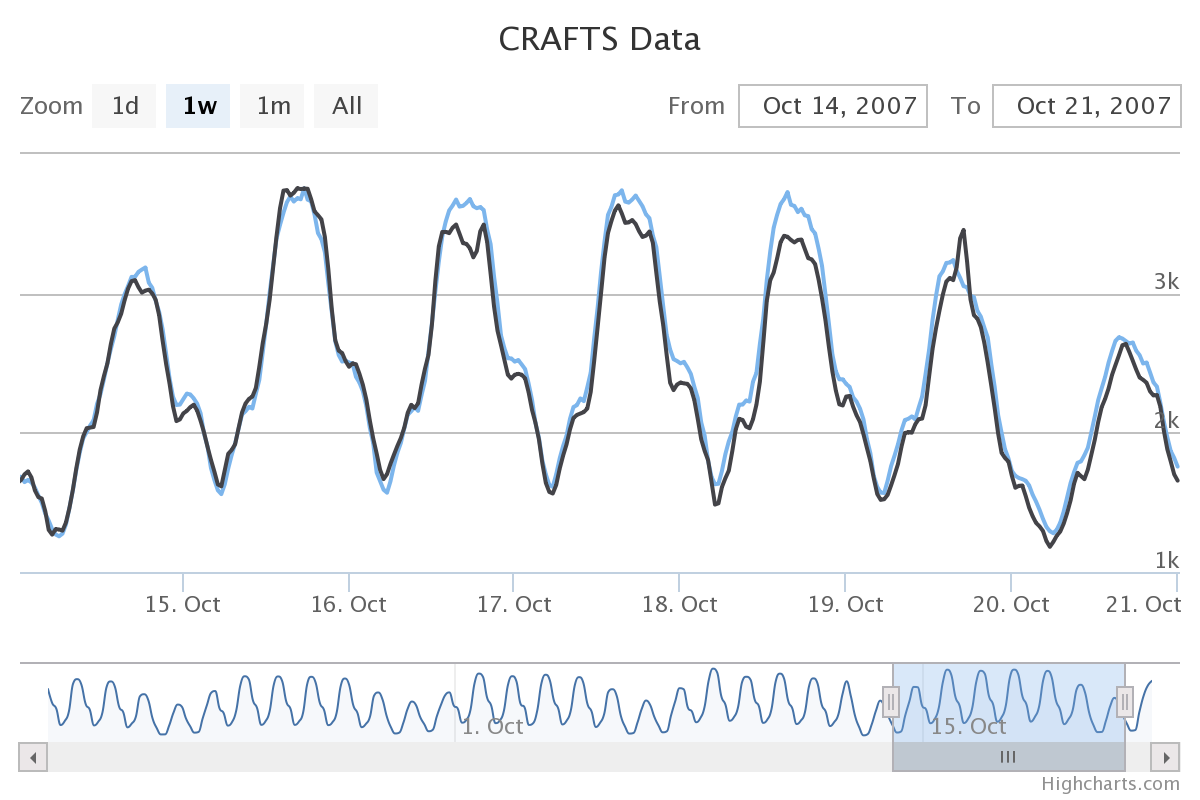
\includegraphics[width=\textwidth]{results/graphs/fft_training_spike.png}
\caption{FFT prediction results for the training spike workload}
\label{fig:fft_ts}
\end{figure}

\begin{table}[H]
\centering
\begin{tabular}{| l | l | l | l | l |}
\hline
Type & \multicolumn{2}{c |}{Regular} & \multicolumn{2}{c |}{Anomalous} \\ \hline
 & RMSD & Percent & RMSD & Percent \\ \hline
Under & 181 & 76.1\% & 3239 & 100.0\% \\ \hline
Over & 61 & 23.9\% & 0 & 0.0\% \\ \hline
Total & 161 & & 3239 & \\ \hline
\end{tabular}
\caption{FFT predictor results for the horizon spike workload}
\end{table}

\begin{figure}[H]
\centering
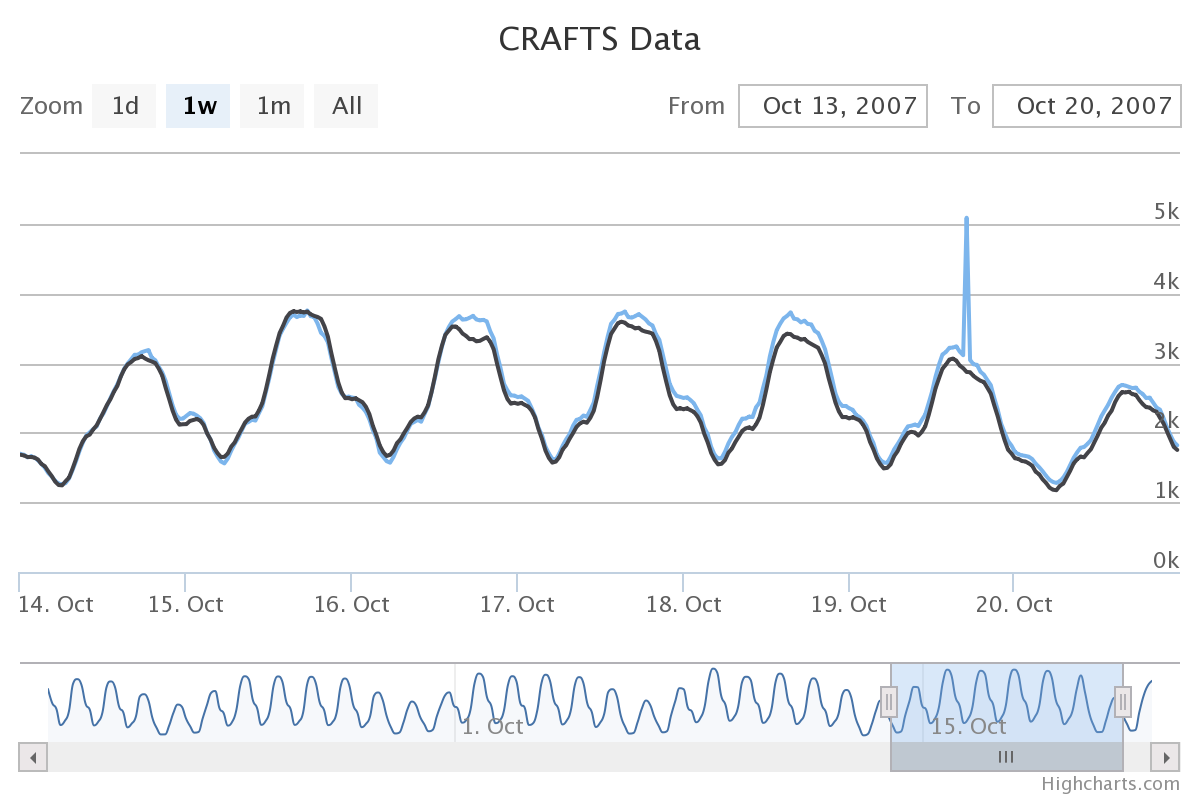
\includegraphics[width=\textwidth]{results/graphs/fft_horizon_spike.png}
\caption{FFT prediction results for the horizon spike workload}
\label{fig:fft_hs}
\end{figure}

\section{Linear Regression}
Since the linear regression predictor uses data spread across multiple weeks, only the final week was used for evaluation and the previous three weeks were used for training.

RESULTS COMING SOON.

\begin{table}[H]
\centering
\begin{tabular}{| l | l | l |}
\hline
Type & RMSD & Percent \\ \hline
Under & 138 & 89.2\% \\ \hline
Over & 32 & 10.8\% \\ \hline
Total & 131 & \\ \hline
\end{tabular}
\caption{Regression predictor results for the baseline workload}
\end{table}

\begin{figure}[H]
\centering
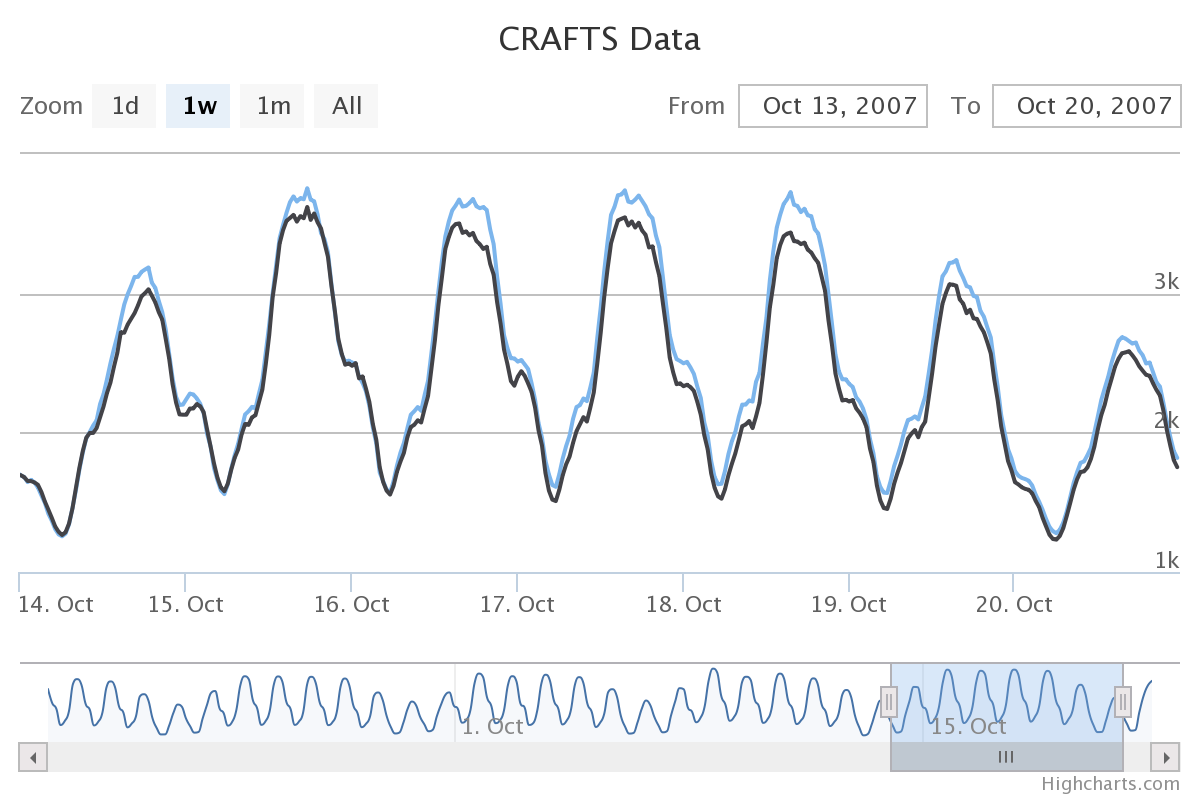
\includegraphics[width=\textwidth]{results/graphs/regression_baseline.png}
\caption{Regression prediction results for the baseline workload}
\label{fig:regression_b}
\end{figure}

\begin{table}[H]
\centering
\begin{tabular}{| l | l | l | l | l |}
\hline
Type & \multicolumn{2}{c |}{Regular} & \multicolumn{2}{c |}{Anomalous} \\ \hline
 & RMSD & Percent & RMSD & Percent \\ \hline
Under & 138 & 89.1\% & 270 & 100.0\% \\ \hline
Over & 32 & 10.9\% & 0 & 0.0\% \\ \hline
Total & 131 & & 270 & \\ \hline
\end{tabular}
\caption{Regression predictor results for the training outage workload}
\end{table}

\begin{figure}[H]
\centering
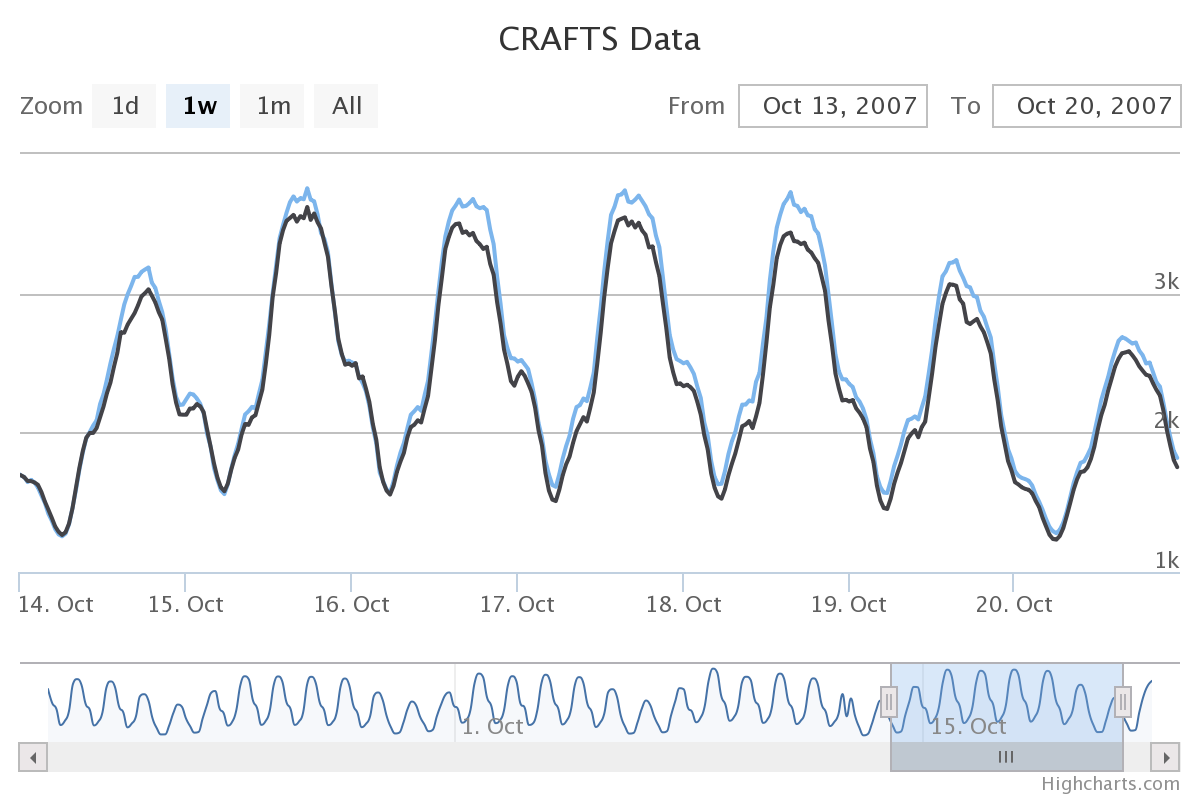
\includegraphics[width=\textwidth]{results/graphs/regression_training_outage.png}
\caption{Regression prediction results for the training outage workload}
\label{fig:regression_to}
\end{figure}

\begin{table}[H]
\centering
\begin{tabular}{| l | l | l | l | l |}
\hline
Type & \multicolumn{2}{c |}{Regular} & \multicolumn{2}{c |}{Anomalous} \\ \hline
 & RMSD & Percent & RMSD & Percent \\ \hline
Under & 138 & 89.0\% & 0 & 0.0\% \\ \hline
Over & 274 & 11.0\% & 2869 & 100.0\% \\ \hline
Total & 159 & & 2869 & \\ \hline
\end{tabular}
\caption{Regression predictor results for the horizon outage workload}
\end{table}

\begin{figure}[H]
\centering
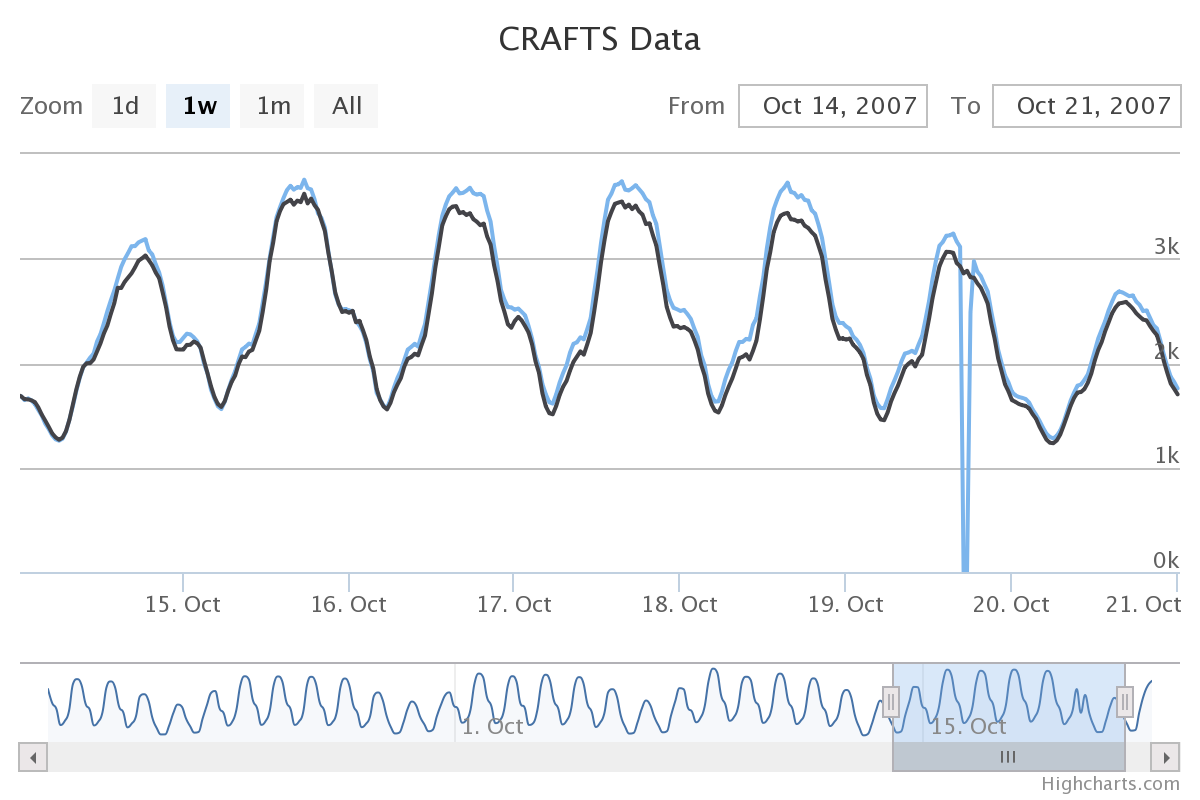
\includegraphics[width=\textwidth]{results/graphs/regression_horizon_outage.png}
\caption{Regression prediction results for the horizon outage workload}
\label{fig:regression_ho}
\end{figure}

\begin{table}[H]
\centering
\begin{tabular}{| l | l | l | l | l |}
\hline
Type & \multicolumn{2}{c |}{Regular} & \multicolumn{2}{c |}{Anomalous} \\ \hline
 & RMSD & Percent & RMSD & Percent \\ \hline
Under & 138 & 89.2\% & 177 & 100.0\% \\ \hline
Over & 32 & 10.8\% & 0 & 0.0\% \\ \hline
Total & 131 & & 177 & \\ \hline
\end{tabular}
\caption{Regression predictor results for the training spike workload}
\end{table}

\begin{figure}[H]
\centering
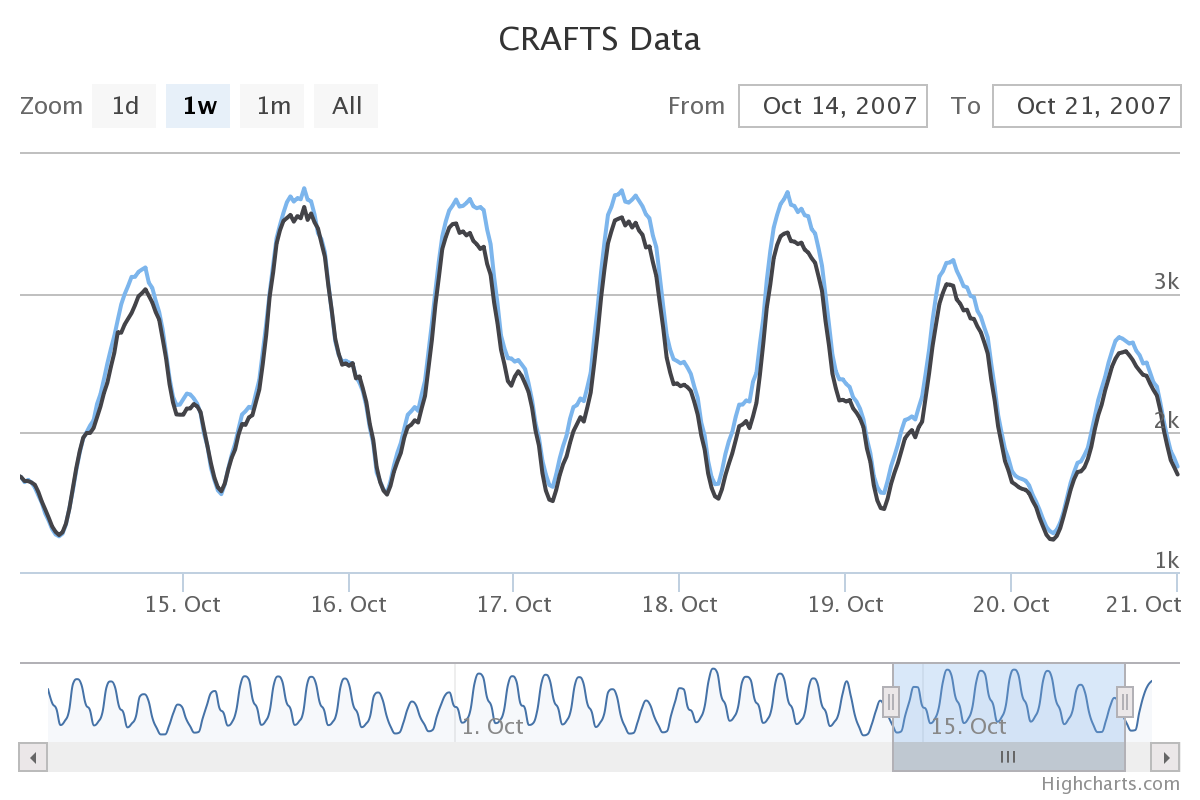
\includegraphics[width=\textwidth]{results/graphs/regression_training_spike.png}
\caption{Regression prediction results for the training spike workload}
\label{fig:regression_ts}
\end{figure}

\begin{table}[H]
\centering
\begin{tabular}{| l | l | l | l | l |}
\hline
Type & \multicolumn{2}{c |}{Regular} & \multicolumn{2}{c |}{Anomalous} \\ \hline
 & RMSD & Percent & RMSD & Percent \\ \hline
Under & 175 & 89.2\% & 3260 & 100.0\% \\ \hline
Over & 32 & 10.8\% & 0 & 0.0\% \\ \hline
Total & 166 & & 3260 & \\ \hline
\end{tabular}
\caption{Regression predictor results for the horizon spike workload}
\end{table}

\begin{figure}[H]
\centering
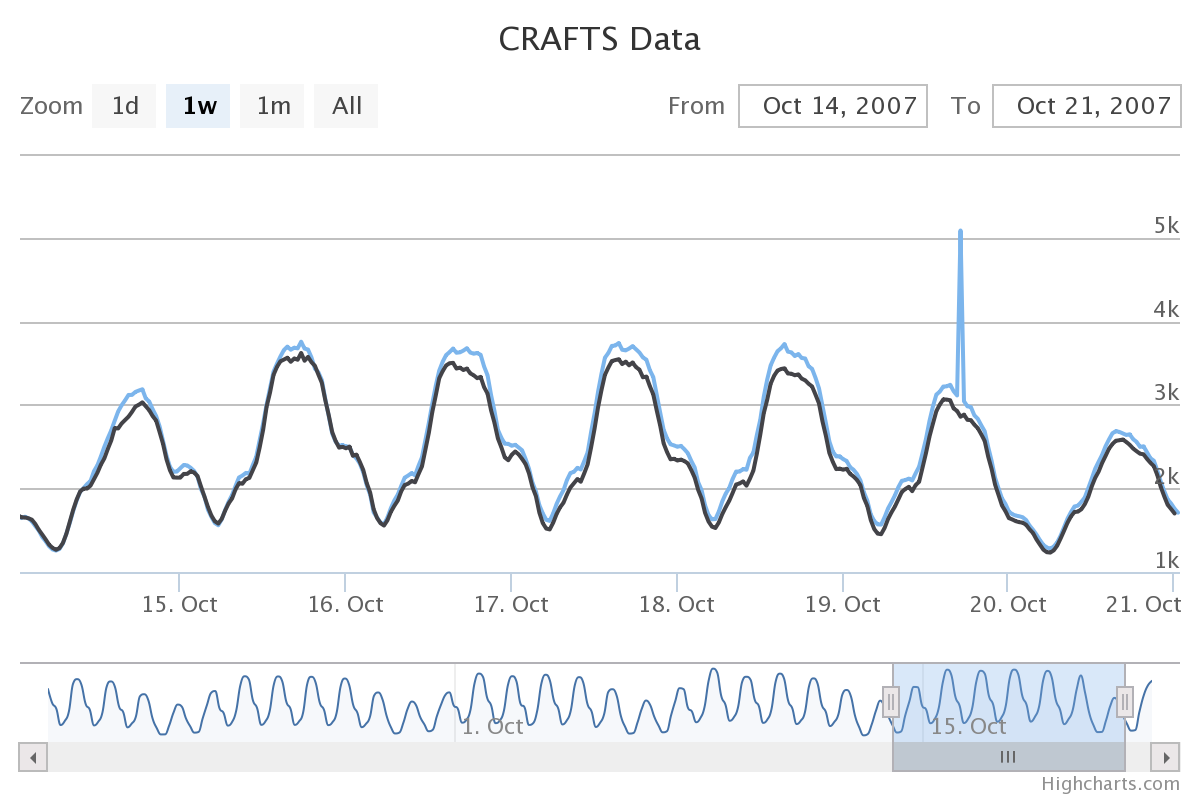
\includegraphics[width=\textwidth]{results/graphs/regression_horizon_spike.png}
\caption{Regression prediction results for the horizon spike workload}
\label{fig:regression_hs}
\end{figure}

\section{Discrete-Time Markov Chain}
The Markov predictor uses the first week of data as a training set and then performs a prediction on the next week. Tuning determined that 85 was the optimal number of buckets to use in this dataset.

While the Markov predictor shows excellent results, its predictions are only accurate in the very short term. This makes it difficult to make optimal scaling decisions in the planner. The Markov predictor is also notably different from the previous predictors in that it does not do any form of translation on the training data. All training data is cummulatively used to generate the probability matrix and then used for predictions. This makes the Markov predictor very resistant to outages and load spikes, while it is still the most accurate predictor so far, both outages and spikes almost double its error.

\begin{table}[H]
\centering
\begin{tabular}{| l | l | l | l | l | l |}
\hline
Type & RMSD & Percent \\ \hline
Under & 27 & 74.0\% \\ \hline
Over & 22 & 26.0\% \\ \hline
Total & 26 & \\ \hline
\end{tabular}
\caption{Markov predictor results for the baseline workload}
\end{table}

% Outage workloads

\begin{table}[H]
\centering
\begin{tabular}{| l | l | l |}
\hline
Type & RMSD & Percent \\ \hline
Under & 52 & 80.8\% \\ \hline
Over & 39 & 19.2\% \\ \hline
Total & 50 & \\ \hline
\end{tabular}
\caption{predictor results for the 10-minute outage workload}
\end{table}

\begin{table}[H]
\centering
\begin{tabular}{| l | l | l |}
\hline
Type & RMSD & Percent \\ \hline
Under & 52 & 80.9\% \\ \hline
Over & 40 & 19.1\% \\ \hline
Total & 50 & \\ \hline
\end{tabular}
\caption{predictor results for the 30-minute outage workload}
\end{table}

\begin{table}[H]
\centering
\begin{tabular}{| l | l | l |}
\hline
Type & RMSD & Percent \\ \hline
Under & 52 & 80.9\% \\ \hline
Over & 39 & 19.1\% \\ \hline
Total & 50 & \\ \hline
\end{tabular}
\caption{predictor results for the 60-minute outage workload}
\end{table}

% Spike workloads

\begin{table}[H]
\centering
\begin{tabular}{| l | l | l |}
\hline
Type & RMSD & Percent \\ \hline
Under & 48 & 76.9\% \\ \hline
Over & 39 & 23.1\% \\ \hline
Total & 46 & \\ \hline
\end{tabular}
\caption{predictor results for the low spike workload}
\end{table}

\begin{table}[H]
\centering
\begin{tabular}{| l | l | l |}
\hline
Type & RMSD & Percent \\ \hline
Under & 48 & 76.9\% \\ \hline
Over & 38 & 23.1\% \\ \hline
Total & 46 & \\ \hline
\end{tabular}
\caption{predictor results for the mid spike workload}
\end{table}

\begin{table}[H]
\centering
\begin{tabular}{| l | l | l |}
\hline
Type & RMSD & Percent \\ \hline
Under & 48 & 76.9\% \\ \hline
Over & 38 & 23.1\% \\ \hline
Total & 46 & \\ \hline
\end{tabular}
\caption{predictor results for the high spike workload}
\end{table}

\section{Exponential Smoothing}
The exponential smoothing predictor was evaluated in the same way as the Markov predictor. It was determined that 0.6 and 0.3 were the optimal values for $\alpha$ and $\beta$, respectively.

The exponential smoothing predictor shares many of the properties of the Markov predictor, but is more susceptible to anomalies in recent temporal data. This is not a problem, however, since the predictions are so short-term they simply accurately reflect the effect of the anomaly as it is occuring.

\begin{table}[H]
\centering
\begin{tabular}{| l | l | l |}
\hline
Type & RMSD & Percent \\ \hline
Under & 42 & 53.2\% \\ \hline
Over & 48 & 46.8\% \\ \hline
Total & 45 & \\ \hline
\end{tabular}
\caption{Exponential smoothing predictor results for the baseline workload}
\end{table}

\begin{figure}[H]
\centering
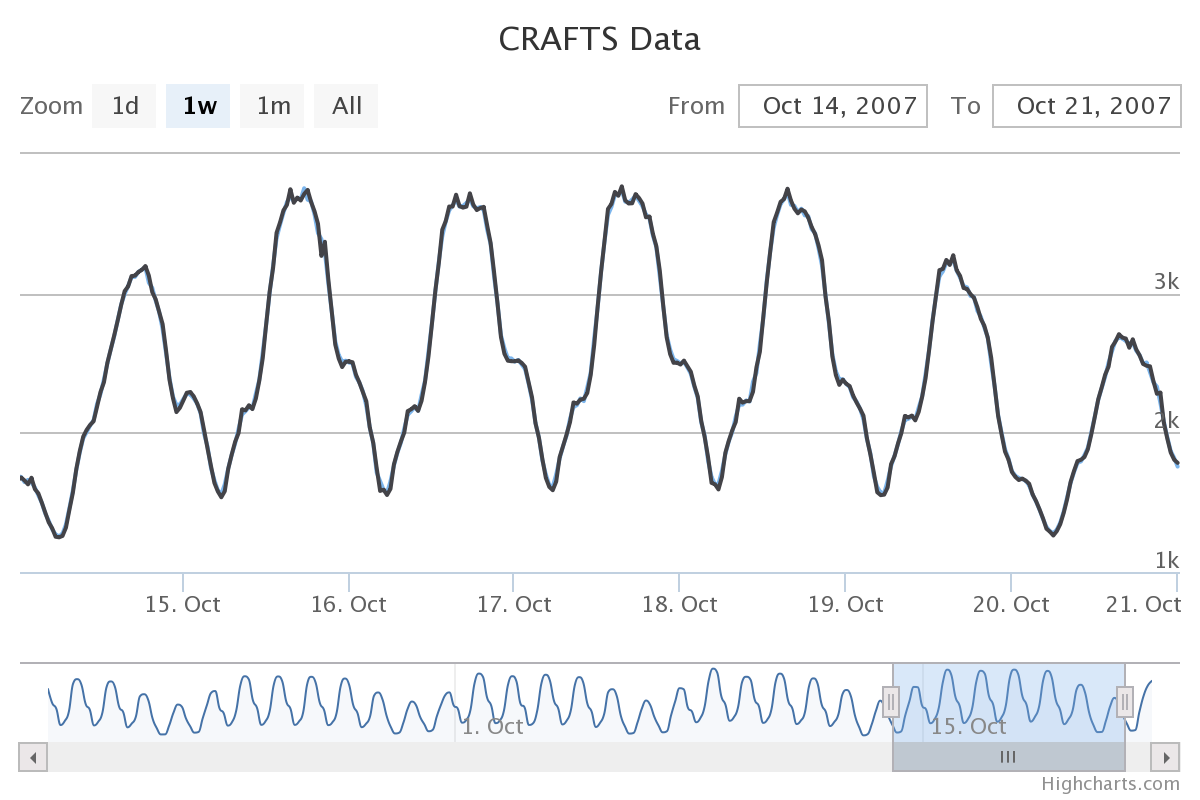
\includegraphics[width=\textwidth]{results/graphs/smoothing_baseline.png}
\caption{Exponential smoothing prediction results for the baseline workload}
\label{fig:smoothing_b}
\end{figure}

\begin{table}[H]
\centering
\begin{tabular}{| l | l | l | l | l |}
\hline
Type & \multicolumn{2}{c |}{Regular} & \multicolumn{2}{c |}{Anomalous} \\ \hline
 & RMSD & Percent & RMSD & Percent \\ \hline
Under & 42 & 53.1\% & 31 & 72.7\% \\ \hline
Over & 48 & 46.9\% & 22 & 27.3\% \\ \hline
Total & 45 & & 29 & \\ \hline
\end{tabular}
\caption{Exponential smoothing predictor results for the training outage workload}
\end{table}

\begin{figure}[H]
\centering
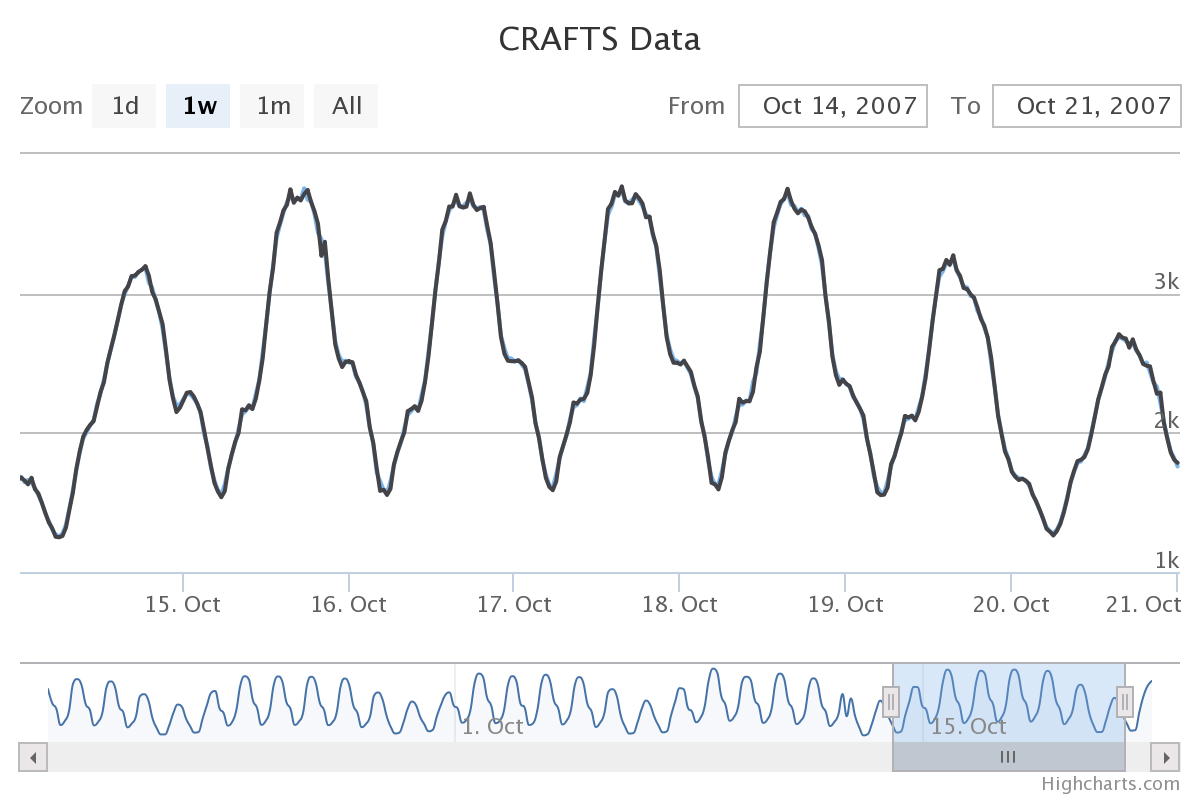
\includegraphics[width=\textwidth]{results/graphs/smoothing_training_outage.png}
\caption{Exponential smoothing prediction results for the training outage workload}
\label{fig:smoothing_to}
\end{figure}

\begin{table}[H]
\centering
\begin{tabular}{| l | l | l | l | l |}
\hline
Type & \multicolumn{2}{c |}{Regular} & \multicolumn{2}{c |}{Anomalous} \\ \hline
 & RMSD & Percent & RMSD & Percent \\ \hline
Under & 165 & 53.0\% & 1216 & 81.8\% \\ \hline
Over & 159 & 47.0\% & 3068 & 18.2\% \\ \hline
Total & 162 & & 1709 & \\ \hline
\end{tabular}
\caption{Exponential smoothing predictor results for the horizon outage workload}
\end{table}

\begin{figure}[H]
\centering
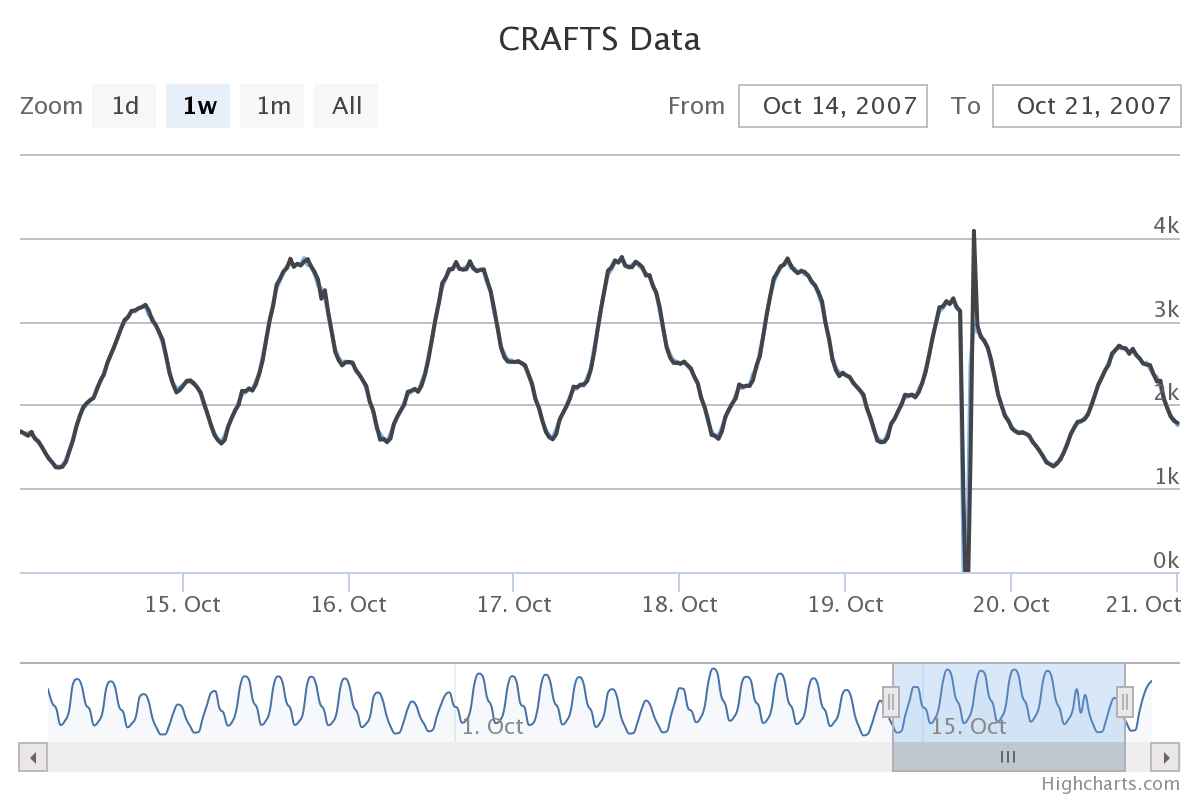
\includegraphics[width=\textwidth]{results/graphs/smoothing_horizon_outage.png}
\caption{Exponential smoothing prediction results for the horizon outage workload}
\label{fig:smoothing_ho}
\end{figure}

\begin{table}[H]
\centering
\begin{tabular}{| l | l | l | l | l |}
\hline
Type & \multicolumn{2}{c |}{Regular} & \multicolumn{2}{c |}{Anomalous} \\ \hline
 & RMSD & Percent & RMSD & Percent \\ \hline
Under & 42 & 53.2\% & 0 & 0.0\% \\ \hline
Over & 48 & 46.8\% & 16 & 100.0\% \\ \hline
Total & 45 & & 16 & \\ \hline
\end{tabular}
\caption{Exponential smoothing predictor results for the training spike workload}
\end{table}

\begin{figure}[H]
\centering
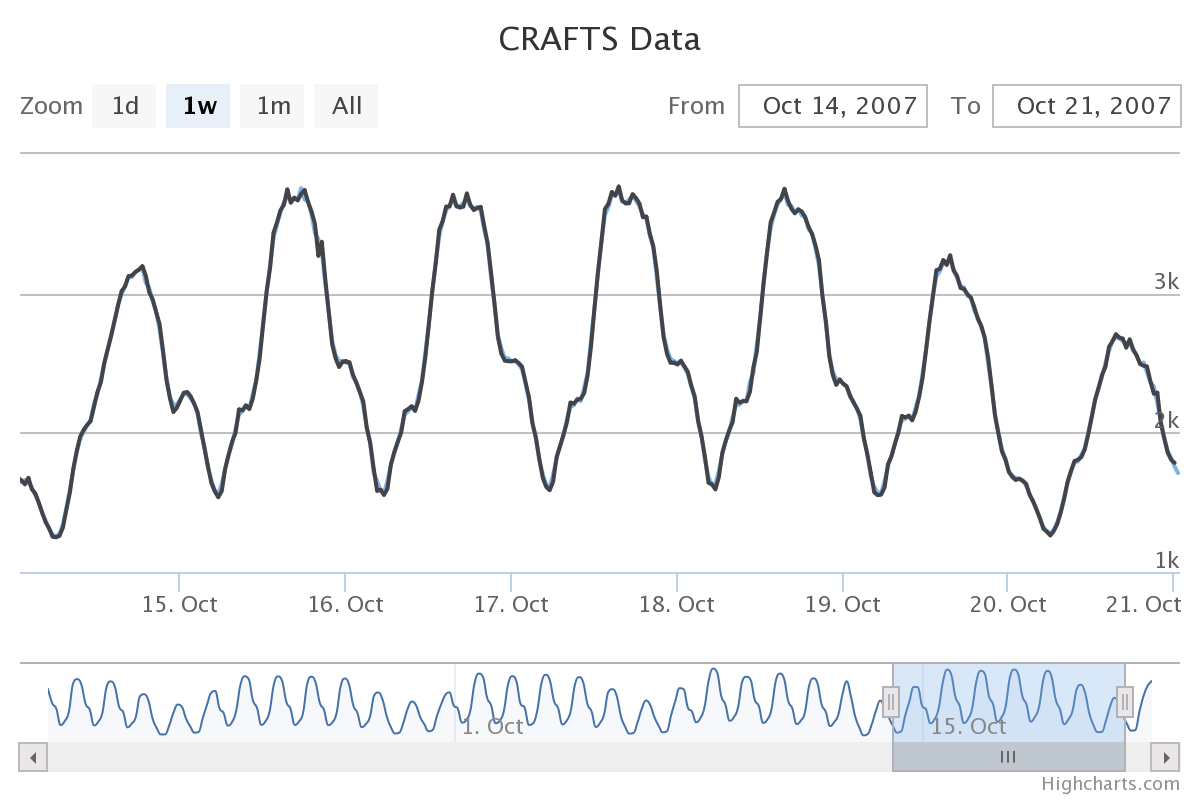
\includegraphics[width=\textwidth]{results/graphs/smoothing_training_spike.png}
\caption{Exponential smoothing prediction results for the training spike workload}
\label{fig:smoothing_ts}
\end{figure}

\begin{table}[H]
\centering
\begin{tabular}{| l | l | l | l | l |}
\hline
Type & \multicolumn{2}{c |}{Regular} & \multicolumn{2}{c |}{Anomalous} \\ \hline
 & RMSD & Percent & RMSD & Percent \\ \hline
Under & 129 & 53.2\% & 3036 & 100.0\% \\ \hline
Over & 277 & 46.8\% & 0 & 0.0\% \\ \hline
Total & 212 & & 3036 & \\ \hline
\end{tabular}
\caption{Exponential smoothing predictor results for the horizon spike workload}
\end{table}

\begin{figure}[H]
\centering
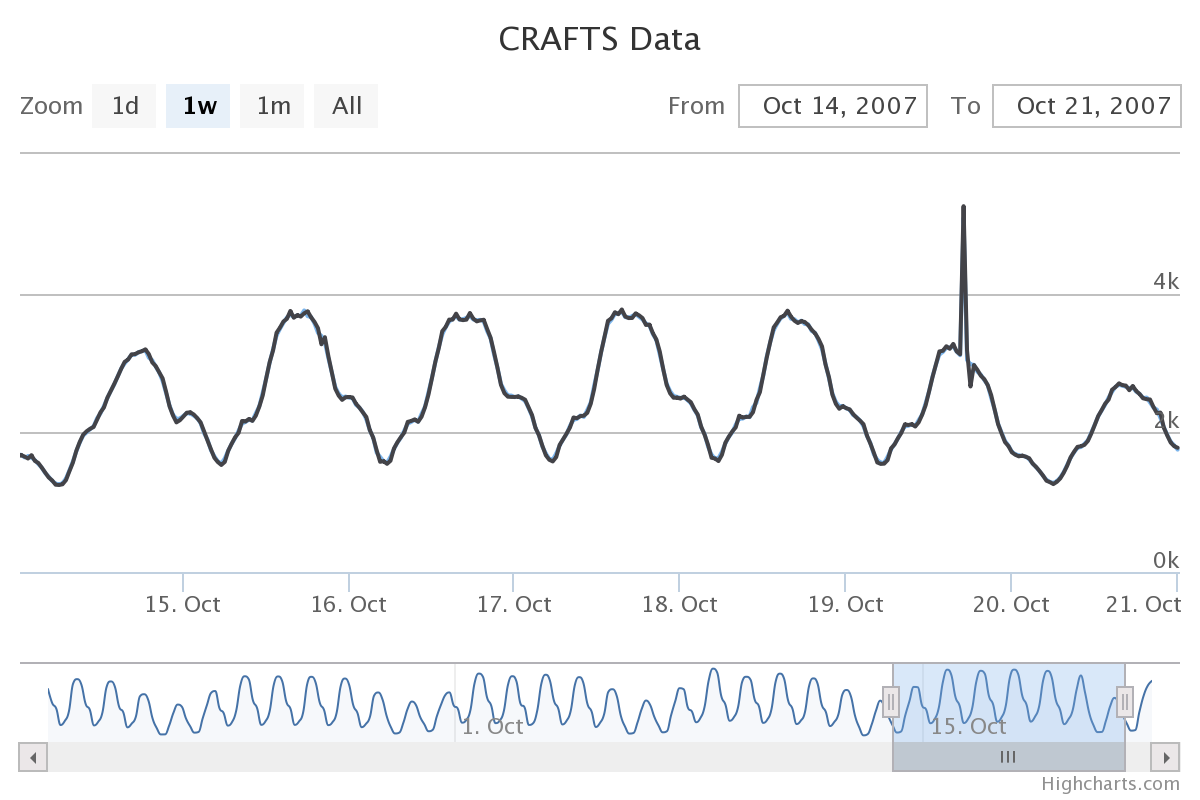
\includegraphics[width=\textwidth]{results/graphs/smoothing_horizon_spike.png}
\caption{Exponential smoothing prediction results for the horizon spike workload}
\label{fig:smoothing_hs}
\end{figure}